\chapter{Annexes}
\section{Annexe 1 : pré-questionnaire et post-questionnaire de l'expérimentation du lancer de fléchettes}\label{annexe1}
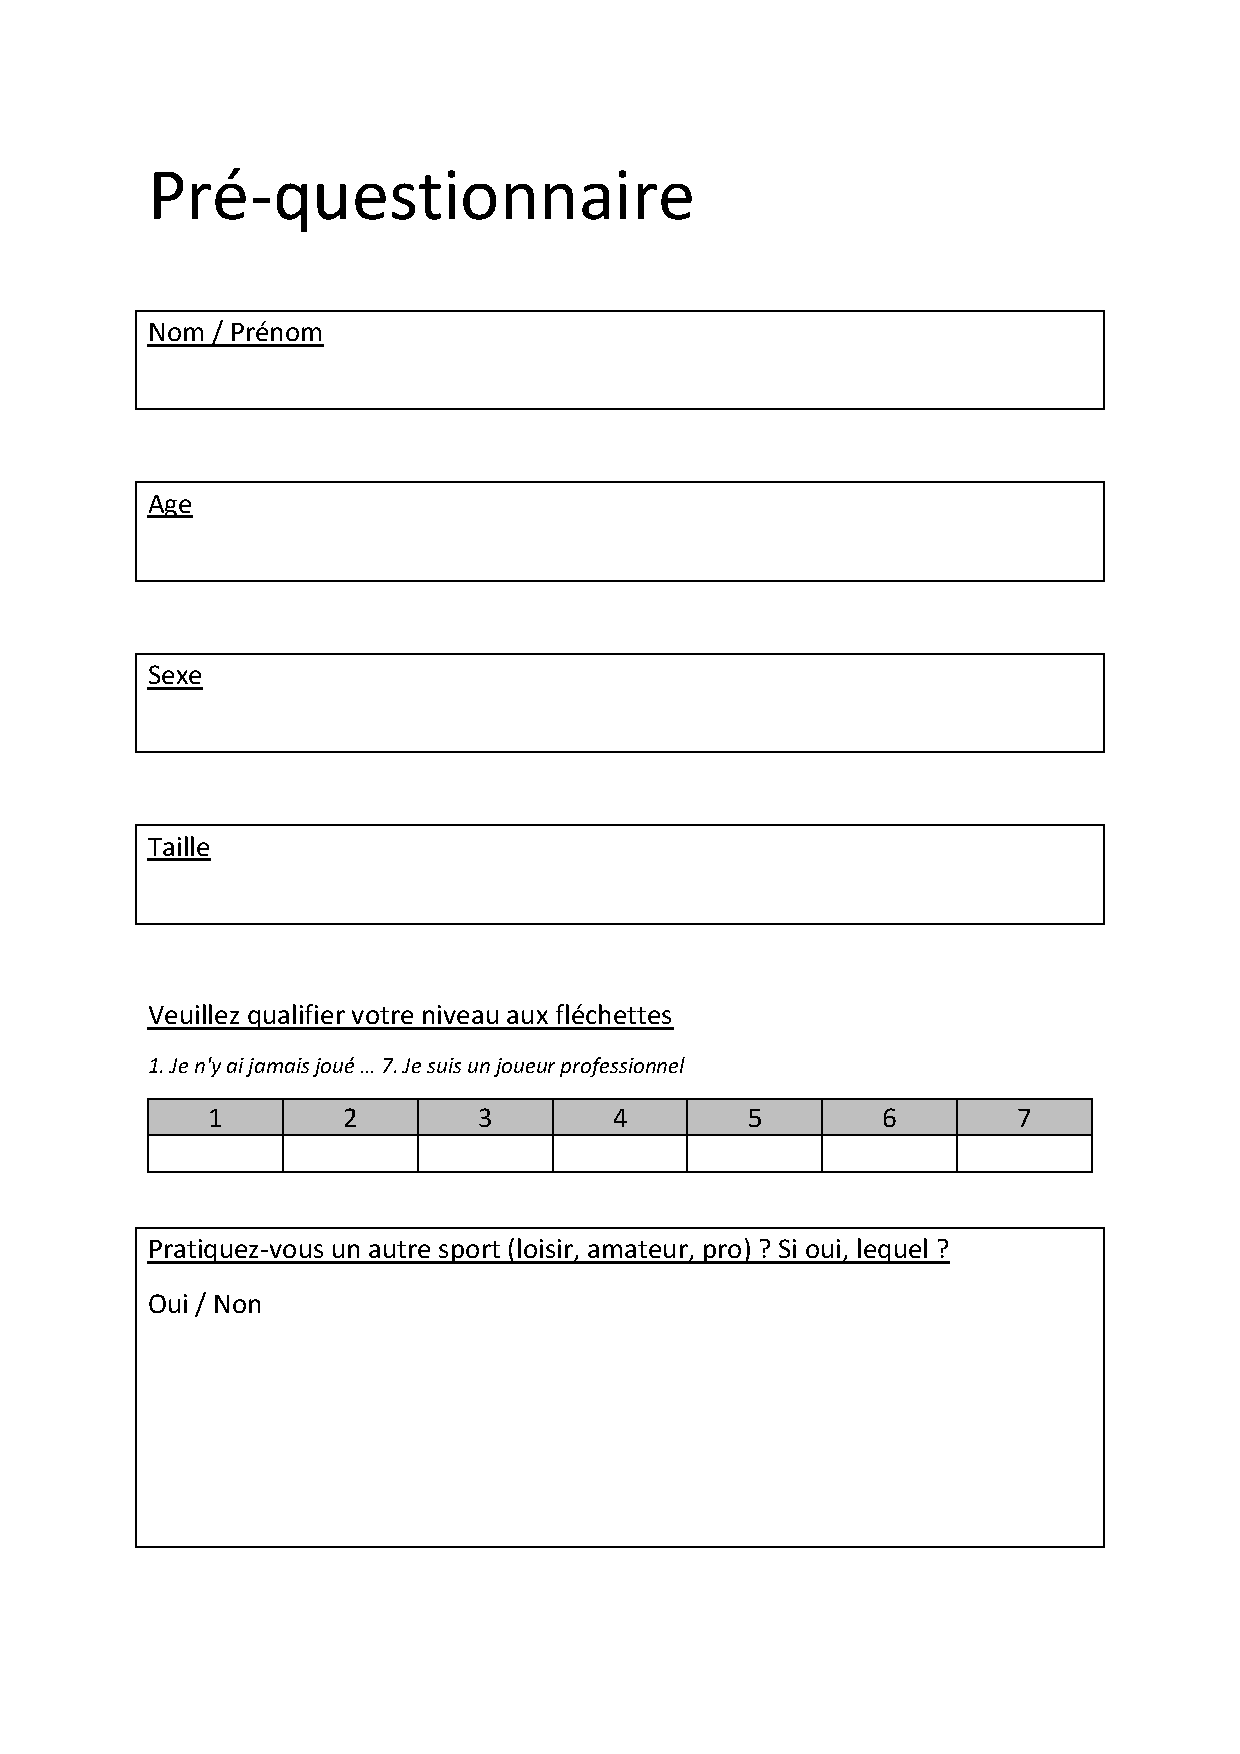
\includepdf[pages=-]{misc/questionnaire.pdf}

\section{Annexe 2 : Tableaux d'analyses complets des résultats de l'expérimentation des fléchettes}\label{annexe2}

\afterpage{
\begin{landscape}
\begin{table}[H]
\centering
\begin{tabular}{ll|cc|ccccc|cccc}
 &  & \multirow{3}{*}{\makecell{Shapiro-Wilk\\($p > 0.05$)}} & \multirow{3}{*}{\makecell{d'Agostino-Pearson\\($p > 0.05$)}} & \multicolumn{5}{c|}{Wilcoxon Signed-Rank ($p < 0.05$)} & \multicolumn{4}{c}{T Test ($p < 0.05$)} \\\cline{5-13}
 &  &  &  & \multicolumn{2}{c}{One tail} & \multicolumn{2}{c}{Two tails} &  & \multirow{2}{*}{One tail} & \multirow{2}{*}{Two tails} & \multirow{2}{*}{t} & \multirow{2}{*}{df} \\\cline{5-9}
 &  &  &  & p-norm & p-exact & p-norm & p-exact & T &  &  &  &  \\\hline
\multirow{3}{*}{Jeu 1-2} & G1 & $1.2329e^{-3}$ & $1.6380e^{-2}$ & 0.0057 & 0.0042 & 0.0115 & 0.0084 & 15 & 0.0044 & 0.0087 & -3.0431 & 14 \\
 & G2 & $1.8799e^{-5}$ & $2.8416e^{-8}$ & 0.0021 & 0.0010 & 0.0041 & 0.0020 & 9 & 0.0023 & 0.0046 & -3.3623 & 14 \\
 & G3 & $3.8069e^{-5}$ & $2.5155e^{-8}$ & 0.0038 & 0.0021 & 0.0076 & 0.0043 & 12.5 & 0.0038 & 0.0076 & -3.1152 & 14 \\\hline
\multirow{3}{*}{Jeu 2-3} & G1 & $9.8712e^{-3}$ & $3.1072e^{-2}$ & 0.0049 & 0.0034 & 0.0098 & 0.0067 & 14 & 0.0016 & 0.0032 & 3.5433 & 14 \\
 & G2 & $3.5333e^{-4}$ & $1.8565e^{-6}$ & 0.1006 & 0.1039 & 0.2013 & 0.2078 & 37 & 0.1151 & 0.2303 & 1.2543 & 14 \\
 & G3 & $7.6972e^{-6}$ & $3.0779e^{-6}$ & 0.5 & 0.4890 & 1 & 0.9780 & 59.5 & 0.2068 & 0.4135 & -0.8427 & 14 \\\hline
\multirow{3}{*}{Jeu 3-4} & G1 & $1.1170e^{-1}$ & $1.6271e^{-1}$ & 0.1743 & 0.1796 & 0.3487 & 0.3591 & 43 & 0.1514 & 0.3028 & 1.0698 & 14 \\
 & G2 & $2.1607e^{-2}$ & $9.0891e^{-2}$ & 0.1221 & 0.1262 & 0.2443 & 0.2524 & 39 & 0.1439 & 0.2877 & 1.1052 & 14 \\
 & G3 & $4.5776e^{-5}$ & $1.1167e^{-4}$ & 0.0144 & 0.0128 & 0.0288 & 0.0256 & 21 & 0.0107 & 0.0214 & 2.5907 & 14 \\\hline
\multirow{3}{*}{Jeu 1-3} & G1 & $2.6205e^{-3}$ & $1.6650e^{-3}$ & 0.1601 & 0.1651 & 0.3202 & 0.3303 & 42 & 0.2149 & 0.4298 & -0.8131 & 14 \\
 & G2 & $3.3477e^{-3}$ & $1.5668e^{-2}$ & 0.1110 & 0.1146 & 0.2220 & 0.2293 & 38 & 0.0662 & 0.1323 & -1.5981 & 14 \\
 & G3 & $5.6502e^{-6}$ & $5.7737e^{-8}$ & 0.01659 & 0.0151 & 0.0332 & 0.0301 & 22 & 0.0131 & 0.0261 & -2.4868 & 14 \\\hline
\multirow{3}{*}{Jeu 2-4} & G1 & $1.2009e^{-2}$ & $3.0490e^{-2}$ & 0.0005 & $9.1553e^{-5}$ & 0.0011 & 0.0002 & 2 & 0.0003 & 0.0005 & 4.4525 & 14 \\
 & G2 & $2.9579e^{-5}$ & $3.8042e^{-8}$ & 0.0073 & 0.0051 & 0.0146 & 0.0102 & 16.5 & 0.0149 & 0.0297 & 2.4199 & 14 \\
 & G3 & $4.2739e^{-5}$ & $3.4339e^{-5}$ & 0.0250 & 0.0240 & 0.0500 & 0.0479 & 25 & 0.1345 & 0.2691 & 1.1508 & 14 \\\hline
\multirow{3}{*}{Jeu 1-4} & G1 & $8.1752e^{-4}$ & $1.2342e^{-4}$ & 0.4660 & 0.4670 & 0.9321 & 0.9341 & 58 & 0.4635 & 0.9270 & -0.0933 & 14 \\
 & G2 & $1.7507e^{-3}$ & $9.6526e^{-4}$ & 0.0864 & 0.0844 & 0.1728 & 0.1688 & 35.5 & 0.1538 & 0.3076 & -1.0589 & 14 \\
 & G3 & $2.1970e^{-5}$ & $5.3364e^{-7}$ & 0.2051 & 0.2106 & 0.4102 & 0.4212 & 45 & 0.1415 & 0.2830 & -1.1164 & 14
\end{tabular}
\caption{Résultats complets des tests statistiques en intragroupe (distance par rapport au centre).}
\end{table}
\end{landscape}}

\begin{table}[H]
\centering
\begin{tabular}{lr|cccc}
 &  & Jeu 1 & Jeu 2 & Jeu 3 & Jeu 4 \\\hline
Shapiro-Wilk ($p > 0.05$) &  & $4.29e^{-5}$ & $1.43e^{-6}$ & $2.06e^{-4}$ & $4.43e^{-5}$  \\
d'Agostino-Pearson ($p > 0.05$) &  &  $1.27e^{-7}$ & $8.38e^{-7}$ & $1.79e^{-5}$ & $1.62e^{-5}$  \\\hline
\multirow{2}{*}{ANOVA ($p < 0.05$)} & $F(2, 42)$ & 0.0907 & 0.7392 & 0.4704 & 0.1307 \\
 & p & 0.9134 & 0.4836 & 0.6280 & 0.8779 \\\hline
\multirow{3}{*}{Pairwise T-test ($p < 0.05$)} & g1 - g2 & 0.9445 & 0.7121 & 0.5244 & 0.6233 \\
 & g1 - g3 & 0.7354 & 0.1902 & 0.3462 & 0.6675 \\
 & g2 - g3 & 0.6659 & 0.4380 & 0.7162 & 0.9650 \\\hline
\multirow{3}{*}{Kruskal-Wallis ($p < 0.05$)} & Chi-square & 0.1875 & 1.8023 & 0.4432 & 0.3937 \\
 & p & 0.9907 & 0.4061 & 0.8012 & 0.8213 \\
 & df & 2 & 2 & 2 & 2 \\\hline
\multirow{3}{*}{Pairwise Mann-Whitney ($p < 0.05$)} & g1 - g2 & 0.9174 & 0.6186 & 0.9357 & 0.6041 \\
 & g1 - g3 & 0.9834 & 0.2210 & 0.5068 & 0.9669 \\
 & g2 - g3 & 0.9339 & 0.3615 & 0.7244 & 0.6041
\end{tabular}
\caption{Résultats complets des tests statistiques en intergroupe (distance par rapport au centre).}
\end{table}

\afterpage{
\begin{landscape}
\begin{table}[H]
\centering
\begin{tabular}{ll|cc|ccccc|cccc}
 &  & \multirow{3}{*}{\makecell{Shapiro-Wilk\\($p > 0.05$)}} & \multirow{3}{*}{\makecell{d'Agostino-Pearson\\($p > 0.05$)}} & \multicolumn{5}{c|}{Wilcoxon Signed-Rank ($p < 0.05$)} & \multicolumn{4}{c}{T Test ($p < 0.05$)} \\\cline{5-13}
 &  &  &  & \multicolumn{2}{c}{One tail} & \multicolumn{2}{c}{Two tails} &  & \multirow{2}{*}{One tail} & \multirow{2}{*}{Two tails} & \multirow{2}{*}{t} & \multirow{2}{*}{df} \\\cline{5-9}
 &  &  &  & p-norm & p-exact & p-norm & p-exact & T &  &  &  &  \\\hline
\multirow{3}{*}{Jeu 1-2} & G1 & $7.6220e^{-6}$ & $9.9203e^{-6}$ & 0.0035 & 0.0021 & 0.0070 & 0.0043 & 12 & 0.0033 & 0.0066 & 3.1837 & 14 \\
 & G2 & 0.0037 & 0.0058 & 0.0285 & 0.0277 & 0.0571 & 0.0553 & 26 & 0.0199 & 0.0398 & 2.2659 & 14 \\
 & G3 & 0.0031 & 0.0348 & 0.2389 & 0.2443 & 0.4777 & 0.4887 & 47 & 0.2783 & 0.5566 & 0.6024 & 14 \\\hline
\multirow{3}{*}{Jeu 2-3} & G1 & $1.836e^{-6}$ & $2.2924e^{-7}$ & 0.1110 & 0.1146 & 0.2220 & 0.2293 & 38 & 0.0729 & 0.1459 & -1.5398 & 14 \\
 & G2 & $1.1879e^{-5}$ & $1.3753e^{-6}$ & 0.2568 & 0.2622 & 0.5136 & 0.5245 & 48 & 0.1927 & 0.3853 & 0.8961 & 14 \\
 & G3 & 0.1079 & 0.0980 & 0.1467 & 0.1514 & 0.2934 & 0.3028 & 41 & 0.3905 & 0.7809 & 0.2835 & 14 \\\hline
\multirow{3}{*}{Jeu 3-4} & G1 & $6.6718e^{-4}$ & 0.0011 & 0.2216 & 0.2271 & 0.4432 & 0.4543 & 46 & 0.1425 & 0.2850 & -1.1117 & 14 \\
 & G2 & $1.3259e^{-6}$ & $1.1894e^{-7}$ & 0.4660 & 0.4670 & 0.9321 & 0.9341 & 58 & 0.4521 & 0.9041 & 0.1226 & 14 \\
 & G3 & 0.0218 & 0.0435 & 0.3774 & 0.3808 & 0.7547 & 0.7615 & 54 & 0.4253 & 0.8506 & -0.1919 & 14 \\\hline
\multirow{3}{*}{Jeu 1-3} & G1 & $5.2763e^{-5}$ & $5.9935e^{-5}$ & 0.0661 & 0.0677 & 0.1323 & 0.1354 & 33 & 0.0406 & 0.0813 & 1.8786 & 14 \\
 & G2 & $1.0753e^{-4}$ & 0.0011 & 0.0144 & 0.0128 & 0.0288 & 0.0256 & 21 & 0.0050 & 0.0100 & 2.9752 & 14 \\
 & G3 & 0.0301 & 0.1060 & 0.2216 & 0.2271 & 0.4432 & 0.4543 & 46 & 0.2134 & 0.4268 & 0.8185 & 14 \\\hline
\multirow{3}{*}{Jeu 2-4} & G1 & $3.6799e^{-5}$ & $2.4848e^{-5}$ & 0.0820 & 0.0844 & 0.1641 & 0.1688 & 35 & 0.0488 & 0.0977 & -1.7748 & 14 \\
 & G2 & $1.6698e^{-4}$ & $1.0856e^{-4}$ & 0.2389 & 0.2243 & 0.4777 & 0.4887 & 47 & 0.1556 & 0.3112 & 1.0506 & 14 \\
 & G3 & 0.0040 & 0.0152 & 0.2216 & 0.2271 & 0.4432 & 0.4543 & 46 & 0.4276 & 0.8552 & 0.1859 & 14 \\\hline
\multirow{3}{*}{Jeu 1-4} & G1 & 0.0017 & 0.0014 & 0.1467 & 0.1514 & 0.2934 & 0.3028 & 41 & 0.2167 & 0.4333 & 0.8067 & 14 \\
 & G2 & $6.7686e^{-4}$ & 0.0029 & 0.0219 & 0.0206 & 0.0438 & 0.0413 & 24 & 0.0128 & 0.0256 & 2.4962 & 14 \\
 & G3 & 0.0020 & 0.0432 & 0.2216 & 0.2271 & 0.4432 & 0.4543 & 46 & 0.2807 & 0.5615 & 0.5948 & 14
\end{tabular}
\caption{Résultats complets des tests statistiques en intragroupe (alignement du bras).}
\end{table}
\end{landscape}}

\begin{table}[H]
\begin{tabular}{lr|cccc}
& & Jeu 1 & Jeu 2 & Jeu 3 & Jeu 4 \\\hline
Shapiro-Wilk ($p > 0.05$) & & $1.0716e^{-4}$ & $1.0445e^{-6}$ & $1.5109e^{-6}$ & $5.0037e^{-5}$ \\
d'Agostino-Pearson ($p > 0.05$) & & $2.0430e^{-4}$ & $4.8091e^{-9}$ & $1.5579e^{-7}$ & $1.6463e^{-4}$ \\\hline
\multirow{2}{*}{ANOVA ($p < 0.05$)} & F (2, 42) & 0.4877 & 0.0820 & 0.5330 & 1.1240 \\
 & p & 0.6175 & 0.9214 & 0.5908 & 0.3346 \\\hline
\multirow{3}{*}{Pairwise T-test ($p < 0.05$)} & g1 - g2 & 0.9972 & 0.9012 & 0.3538 & 0.1728 \\
 & g1 - g3 & 0.3651 & 0.6990 & 0.5972 & 0.4170 \\
 & g2 - g3 & 0.3724 & 0.7628 & 0.5855 & 0.4774 \\\hline
\multirow{3}{*}{Kruskal-Wallis ($p < 0.05$)} & Chi-square & 0.4970 & 1.9223 & 3.2518 & 2.5979 \\
 & p & 0.78000 & 0.3824 & 0.1967 & 0.2728 \\
 & df & 2 & 2 & 2 & 2 \\\hline
\multirow{3}{*}{Mann-Whitney ($p < 0.05$)} & g1 - g2 & 0.9339 & 0.6783 & 0.0890 & 0.1585 \\
 & g1 - g3 & 0.5338 & 0.1466 & 0.8357 & 0.5614 \\
 & g2 - g3 & 0.5897 & 0.4807 & 0.1844 & 0.2290
\end{tabular}
\caption{Résultats complets des tests statistiques en intergroupe (alignement du bras).}
\end{table}

\afterpage{
\begin{landscape}
\begin{table}[H]
\centering
\begin{tabular}{ll|cc|ccccc|cccc}
 &  & \multirow{3}{*}{\makecell{Shapiro-Wilk\\($p > 0.05$)}} & \multirow{3}{*}{\makecell{d'Agostino-Pearson\\($p > 0.05$)}} & \multicolumn{5}{c|}{Wilcoxon Signed-Rank ($p < 0.05$)} & \multicolumn{4}{c}{T Test ($p < 0.05$)} \\\cline{5-13}
 &  &  &  & \multicolumn{2}{c}{One tail} & \multicolumn{2}{c}{Two tails} &  & \multirow{2}{*}{One tail} & \multirow{2}{*}{Two tails} & \multirow{2}{*}{t} & \multirow{2}{*}{df} \\\cline{5-9}
 &  &  &  & p-norm & p-exact & p-norm & p-exact & T &  &  &  &  \\\hline
\multirow{3}{*}{Jeu 1-2} & G1 & 0.0042 & $9.6266e^{-4}$ & $6.6602e^{-4}$ & $1.5259e^{-4}$ & 0.0013 & $3.0518e^{-4}$ & 3 & $3.9473e^{-4}$ & $7.8946e^{-4}$ & 4.2621 & 14 \\
 & G2 & 0.0244 & 0.0162 & $9.8276e^{-4}$ & $3.0518e^{-4}$ & 0.0020 & $6.1035e^{-4}$ & 5 & 0.0026 & 0.0052 & 3.3014 & 14 \\
 & G3 & $5.4414e^{-4}$ & 0.0030 & $4.4595e^{-4}$ & $6.1035e^{-5}$ & $8.9190e^{-4}$ & $1.2207e^{-4}$ & 1 & $4.2438e^{-5}$ & $8.4875e^{-5}$ & 5.4545 & 14 \\\hline
\multirow{3}{*}{Jeu 2-3} & G1 & 0.1226 & 0.0587 & 0.3351 & 0.3394 & 0.6701 & 0.6788 & 52 & 0.3617 & 0.7235 & -0.3910 & 14 \\
 & G2 & 0.0467 & 0.1537 & 0.0738 & 0.0757 & 0.1475 & 0.1514 & 34 & 0.0482 & 0.0964 & 1.7820 & 14 \\
 & G3 & $4.4354e^{-5}$ & $8.3421e^{-5}$ & 0.0661 & 0.0677 & 0.1323 & 0.1354 & 33 & 0.0897 & 0.1794 & 1.4131 & 14 \\\hline
\multirow{3}{*}{Jeu 3-4} & G1 & 0.1857 & 0.3624 & 0.4887 & 0.4890 & 0.9773 & 0.9780 & 59 & 0.4712 & 0.9425 & -0.0735 & 14 \\
 & G2 & 0.0219 & 0.0302 & 0.3991 & 0.4020 & 0.7983 & 0.8039 & 55 & 0.4998 & 0.9995 & $-5.9803e^{-4}$ & 14 \\
 & G3 & $4.3685e^{-4}$ & 0.0050 & 0.0416 & 0.0416 & 0.0832 & 0.0832 & 29 & 0.0499 & 0.0997 & -1.7628 & 14 \\\hline
\multirow{3}{*}{Jeu 1-3} & G1 & 0.0051 & $4.9284e^{-4}$ & $3.6326e^{-4}$ & $3.0518e^{-5}$ & $7.2651e^{-4}$ & $6.1035e^{-5}$ & 0 & $4.8085e^{-4}$ & $9.6171e^{-4}$ & 4.1605 & 14 \\
 & G2 & 0.0038 & 0.0728 & 0.0038 & 0.0021 & 0.0076 & 0.0043 & 12.5 & 0.0018 & 0.0036 & 3.4882 & 14 \\
 & G3 & $1.8900e^{-4}$ & $3.5421e^{-4}$ & 0.0014 & $5.7983e^{-4}$ & 0.0029 & 0.0012 & 7 & $1.9457e^{-4}$ & $3.8914e^{-4}$ & 4.6306 & 14 \\\hline
\multirow{3}{*}{Jeu 2-4} & G1 & 0.1147 & 0.1421 & 0.2947 & 0.2997 & 0.5895 & 0.5995 & 50 & 0.3837 & 0.7675 & -0.3015 & 14 \\
 & G2 & 0.0984 & 0.2806 & 0.0285 & 0.0277 & 0.0571 & 0.0554 & 26 & 0.0263 & 0.0525 & 2.1182 & 14 \\
 & G3 & $1.0791e^{-4}$ & $3.3700e^{-4}$ & 0.4435 & 0.4452 & 0.8871 & 0.8904 & 57 & 0.3351 & 0.6702 & 0.4350 & 14 \\\hline
\multirow{3}{*}{Jeu 1-4} & G1 & 0.0055 & $7.2099e^{-4}$ & $6.6602e^{-4}$ & $1.5259e^{-4}$ & 0.0013 & $3.0518e^{-4}$ & 3 & $5.2838e^{-4}$ & 0.0011 & 4.1121 & 14 \\
 & G2 & 0.0027 & 0.0791 & $6.6602e^{-4}$ & $1.5259e^{-4}$ & 0.0013 & $3.0518e^{-4}$ & 3 & 0.0015 & 0.0030 & 3.5854 & 14 \\
 & G3 & $3.6654e^{-4}$ & $4.8664e^{-4}$ & $5.4581e^{-4}$ & $9.1553e^{-5}$ & 0.0011 & $1.8311e^{-4}$ & 2 & $1.1619e^{-4}$ & $2.3239e^{-4}$ & 4.9044 & 14
\end{tabular}
\caption{Résultats complets des tests statistique en intragroupe (mouvement du coude).}
\end{table}
\end{landscape}}

\begin{table}[H]
\begin{tabular}{lr|cccc}
& & Jeu 1 & Jeu 2 & Jeu 3 & Jeu 4 \\\hline
Shapiro-Wilk ($p > 0.05$) & & 0.0291 & $7.8979e^{-4}$ & 0.0224 & $1.5553e^{-3}$ \\
d'Agostino-Pearson ($p > 0.05$) & & 0.0324 & $2.4829e^{-4}$ & 0.1270 & 0.0105 \\\hline
\multirow{2}{*}{ANOVA ($p < 0.05$)} & F (2, 42) & 0.5691 & 0.0828 & 0.4350 & 0.5286 \\
 & p & 0.5703 & 0.9207 & 0.6501 & 0.5933 \\\hline
\multirow{3}{*}{Pairwise T-test ($p < 0.05$)} & g1 - g2 & 0.2861 & 0.7085 & 0.3233 & 0.3562 \\
 & g1 - g3 & 0.7416 & 0.7254 & 0.6167 & 0.9693 \\
 & g2 - g3 & 0.4787 & 0.9455 & 0.6993 & 0.3870 \\\hline
\multirow{3}{*}{Kruskal-Wallis ($p < 0.05$)} & Chi-square & 0.9793 & 0.2319 & 1.0321 & 0.5969 \\
 & p & 0.6128 & 0.8905 & 0.5969 & 0.4460 \\
 & df & 2 & 2 & 2 & 2 \\\hline
\multirow{3}{*}{Mann-Whitney ($p < 0.05$)} & g1 - g2 & 0.4306 & 0.7715 & 0.4068 & 0.2134 \\
 & g1 - g3 & 0.4807 & 0.9339 & 0.4068 & 0.6187 \\
 & g2 - g3 & 0.5614 & 0.6187 & 0.6783 & 0.4807
\end{tabular}
\caption{Résultats complets des tests statistiques en intergroupe (mouvement du coude).}
\end{table}

\afterpage{
\begin{landscape}
\begin{table}[H]
\centering
\begin{tabular}{ll|cc|ccccc|cccc}
 &  & \multirow{3}{*}{\makecell{Shapiro-Wilk\\($p > 0.05$)}} & \multirow{3}{*}{\makecell{d'Agostino-Pearson\\($p > 0.05$)}} & \multicolumn{5}{c|}{Wilcoxon Signed-Rank ($p < 0.05$)} & \multicolumn{4}{c}{T Test ($p < 0.05$)} \\\cline{5-13}
 &  &  &  & \multicolumn{2}{c}{One tail} & \multicolumn{2}{c}{Two tails} &  & \multirow{2}{*}{One tail} & \multirow{2}{*}{Two tails} & \multirow{2}{*}{t} & \multirow{2}{*}{df} \\\cline{5-9}
 &  &  &  & p-norm & p-exact & p-norm & p-exact & T &  &  &  &  \\\hline
\multirow{3}{*}{Jeu 1-2} & G1 & 0.01367 & 0.1962 & 0.0219 & 0.2006 & 0.0438 & 0.0413 & 24 & 0.0226 & 0.0452 & 2.1984 & 14 \\
 & G2 & 0.01983 & 0.2513 & 0.0124 & 0.0108 & 0.0249 & 0.0215 & 20 & 0.0596 & 0.1192 & 1.6598 & 14 \\
 & G3 & 0.0039 & 0.0040 & 0.2755 & 0.2807 & 0.5509 & 0.5614 & 49 & 0.1727 & 0.3453 & 0.9766 & 14 \\\hline
\multirow{3}{*}{Jeu 2-3} & G1 & 0.0573 & 0.1503 & 0.1743 & 0.1796 & 0.3487 & 0.3591 & 43 & 0.3370 & 0.6741 & -0.4295 & 14 \\
 & G2 & $4.5656e^{-4}$ & $5.7237e^{-5}$ & 0.2568 & 0.2622 & 0.5136 & 0.5245 & 48 & 0.2265 & 0.4531 & -0.7718 & 14 \\
 & G3 & 0.4498 & 0.6546 & 0.1340 & 0.1384 & 0.2681 & 0.2768 & 40 & 0.1105 & 0.2209 & -1.2812 & 14 \\\hline
\multirow{3}{*}{Jeu 3-4} & G1 & 0.1498 & 0.7804 & 0.3774 & 0.3808 & 0.7547 & 0.7615 & 54 & 0.2455 & 0.4911 & 0.7071 & 14 \\
 & G2 & $6.2827e^{-5}$ & $4.9680e^{-7}$ & 0.0029 & 0.0017 & 0.0059 & 0.0034 & 11 & 0.0065 & 0.0129 & 2.8463 & 14 \\
 & G3 & 0.3668 & 0.6230 & 0.3774 & 0.3808 & 0.7547 & 0.7615 & 54 & 0.2817 & 0.5635 & 0.5917 & 14 \\\hline
\multirow{3}{*}{Jeu 1-3} & G1 & 0.2698 & 0.3782 & 0.0910 & 0.0938 & 0.1820 & 0.1876 & 36 & 0.0739 & 0.1478 & 1.5322 & 14 \\
 & G2 & 0.0028 & $3.7064e^{-4}$ & 0.0191 & 0.0177 & 0.0381 & 0.0353 & 23 & 0.1562 & 0.3125 & 1.0477 & 14 \\
 & G3 & 0.0147 & 0.0110 & 0.4435 & 0.4452 & 0.8871 & 0.8904 & 57 & 0.3199 & 0.6398 & 0.4784 & 14 \\\hline
\multirow{3}{*}{Jeu 2-4} & G1 & 0.0891 & 0.1857 & 0.2051 & 0.2106 & 0.4102 & 0.4212 & 45 & 0.4212 & 0.8424 & -0.2025 & 14 \\
 & G2 & 0.0119 & 0.0066 & 0.0057 & 0.0042 & 0.0115 & 0.0084 & 15 & 0.0038 & 0.0076 & 3.1159 & 14 \\
 & G3 & 0.2446 & 0.4480 & 0.3774 & 0.3808 & 0.7547 & 0.7615 & 54 & 0.3671 & 0.7341 & -0.3465 & 14 \\\hline
\multirow{3}{*}{Jeu 1-4} & G1 & 0.9655 & 0.4871 & 0.0738 & 0.0757 & 0.1475 & 0.1514 & 34 & 0.0530 & 0.1061 & 1.7275 & 14 \\
 & G2 & 0.2532 & 0.3443 & 0.0035 & 0.0021 & 0.0070 & 0.0043 & 12 & 0.0030 & 0.0061 & 3.2280 & 14 \\
 & G3 & 0.0161 & 0.0243 & 0.2389 & 0.2443 & 0.4777 & 0.4887 & 47 & 0.2189 & 0.4378 & 0.7987 & 14
\end{tabular}
\caption{Résultats complets des tests statistiques en intragroupe (lancer de type javelot).}
\end{table}
\end{landscape}}

\begin{table}[H]
\begin{tabular}{lr|cccc}
& & Jeu 1 & Jeu 2 & Jeu 3 & Jeu 4 \\\hline
Shapiro-Wilk ($p > 0.05$) & & 0.1308 & $2.1392e^{-4}$ & $5.2743e^{-5}$ & 0.0902 \\
d'Agostino-Pearson ($p > 0.05$) &  & 0.0872 & $2.2381e^{-4}$ & $1.3488e^{-7}$ & 0.1036 \\\hline
\multirow{2}{*}{ANOVA ($p < 0.05$)} & F (2, 42) & 2.6135 & 0.8371 & 0.6180 & 1.4252 \\
 & p & 0.0852 & 0.4400 & 0.5438 & 0.2518 \\\hline
\multirow{3}{*}{Pairwise T-test ($p < 0.05$)} & g1 - g2 & 0.9922 & 0.9792 & 0.9484 & 0.1667 \\
 & g1 - g3 & 0.0619 & 0.2552 & 0.2491 & 0.2280 \\
 & g2 - g3 & 0.0374 & 0.2017 & 0.3335 & 0.6985 \\\hline
\multirow{3}{*}{Kruskal-Wallis ($p < 0.05$)} & Chi-square & 5.2877 & 0.8371 & 0.4924 & 1.9695 \\
 & p & 0.0711 & 0.6580 & 0.7818 & 0.3735 \\
 & df & 2 & 2 & 2 & 2 \\\hline
\multirow{3}{*}{Mann-Whitney ($p < 0.05$)} & g1 - g2 & 0.7400 & 0.8682 & 0.7715 & 0.2455 \\
 & g1 - g3 & 0.0512 & 0.5338 & 0.4068 & 0.2998 \\
 & g2 - g3 & 0.0512 & 0.3837 & 1 & 0.4807
\end{tabular}
\caption{Résultats complets des tests statistiques en intergroupe (lancer de type javelot).}
\end{table}

\afterpage{
\begin{landscape}
\begin{table}[H]
\centering
\begin{tabular}{ll|cc|ccccc|cccc}
 &  & \multirow{3}{*}{\makecell{Shapiro-Wilk\\($p > 0.05$)}} & \multirow{3}{*}{\makecell{d'Agostino-Pearson\\($p > 0.05$)}} & \multicolumn{5}{c|}{Wilcoxon Signed-Rank ($p < 0.05$)} & \multicolumn{4}{c}{T Test ($p < 0.05$)} \\\cline{5-13}
 &  &  &  & \multicolumn{2}{c}{One tail} & \multicolumn{2}{c}{Two tails} &  & \multirow{2}{*}{One tail} & \multirow{2}{*}{Two tails} & \multirow{2}{*}{t} & \multirow{2}{*}{df} \\\cline{5-9}
 &  &  &  & p-norm & p-exact & p-norm & p-exact & T &  &  &  &  \\\hline
\multirow{3}{*}{Jeu 1-2} & G1 & 0.0027 & 0.0181 & $8.1026e^{-4}$ & $2.1362e^{-4}$ & 0.0016 & $4.2725e^{-4}$ & 4 & $3.6924e^{-4}$ & $7.3848e^{-4}$ & 4.2965 & 14 \\
 & G2 & $8.8603e^{-4}$ & 0.0032 & 0.0592 & 0.0603 & 0.1183 & 0.1205 & 32 & 0.0166 & 0.0332 & 2.3622 & 14 \\
 & G3 & 0.0013 & 0.0135 & $9.8276e^{-4}$ & $3.0518e^{-4}$ & 0.0020 & $6.1035e^{-4}$ & 5 & $1.1282e^{-4}$ & $2.2564e^{-4}$ & 4.9202 & 14 \\\hline
\multirow{3}{*}{Jeu 2-3} & G1 & 0.0772 & 0.2829 & 0.4212 & 0.4235 & 0.8425 & 0.8469 & 56 & 0.4993 & 0.9986 & 0.0018 & 14 \\
 & G2 & 0.0243 & 0.1288 & 0.0469 & 0.047 & 0.0938 & 0.0946 & 30 & 0.0336 & 0.0671 & 1.9845 & 14 \\
 & G3 & $1.022e^{-4}$ & $8.5817e^{-5}$ & 0.2755 & 0.2807 & 0.5509 & 0.5614 & 49 & 0.1708 & 0.3416 & 0.9845 & 14 \\\hline
\multirow{3}{*}{Jeu 3-4} & G1 & 0.0715 & 0.4646 & 0.3351 & 0.3394 & 0.6701 & 0.6788 & 52 & 0.4445 & 0.8891 & 0.1420 & 14 \\
 & G2 & 0.0150 & 0.0968 & 0.4435 & 0.4452 & 0.8871 & 0.8904 & 57 & 0.4438 & 0.8875 & -0.1440 & 14 \\
 & G3 & 0.0024 & 0.0062 & 0.0592 & 0.0603 & 0.1183 & 0.1205 & 32 & 0.0349 & 0.0698 & -1.9630 & 14 \\\hline
\multirow{3}{*}{Jeu 1-3} & G1 & 0.0018 & 0.0110 & $9.8276e^{-4}$ & $3.0518e^{-4}$ & 0.0020 & $6.1035e^{-4}$ & 5 & $8.0872e^{-4}$ & 0.0016 & 3.8950 & 14 \\
 & G2 & $1.2268e^{-4}$ & 0.0011 & 0.0219 & 0.0206 & 0.0438 & 0.0413 & 24 & 0.0084 & 0.0168 & 2.7140 & 14 \\
 & G3 & $5.7966e^{-4}$ & 0.0021 & 0.0014 & $5.7983e^{-4}$ & 0.0029 & 0.0012 & 7 & $4.0077e^{-4}$ & $8.0155e^{-4}$ & 4.2542 & 14 \\\hline
\multirow{3}{*}{Jeu 2-4} & G1 & 0.0376 & 0.3332 & 0.4660 & 0.4670 & 0.9321 & 0.9341 & 58 & 0.4633 & 0.9266 & 0.0937 & 14 \\
 & G2 & 0.0352 & 0.1804 & 0.0219 & 0.0206 & 0.0438 & 0.0413 & 24 & 0.0166 & 0.0332 & 2.3622 & 14 \\
 & G3 & $3.0491e^{-4}$ & $2.4575e^{-4}$ & 0.4435 & 0.4452 & 0.8871 & 0.8904 & 57 & 0.4895 & 0.9790 & 0.0268 & 14 \\\hline
\multirow{3}{*}{Jeu 1-4} & G1 & 0.0023 & 0.0137 & 0.0014 & $5.7983e^{-4}$ & 0.0029 & 0.0012 & 7 & $6.9935e^{-4}$ & 0.0014 & 3.9689 & 14 \\
 & G2 & $1.2774e^{-4}$ & $7.9260e^{-4}$ & 0.0191 & 0.0177 & 0.0382 & 0.0353 & 23 & 0.0081 & 0.0163 & 2.7300 & 14 \\
 & G3 & 0.0010 & 0.0026 & 0.0017 & $7.6294e^{-4}$ & 0.0034 & 0.0015 & 8 & $2.1431e^{-4}$ & $4.2861e^{-4}$ & 4.5798 & 14
\end{tabular}
\caption{Résultats complets des tests statistiques en intragroupe (corps penché).}
\end{table}
\end{landscape}}

\begin{table}[H]
\begin{tabular}{lr|cccc}
 &  & Jeu 1 & Jeu 2 & Jeu 3 & Jeu 4 \\\hline
Shapiro-Wilk ($p > 0.05$) &  & 0.0050 & $6.3275e^{-5}$ & 0.0017 & $7.1272e^{-4}$ \\
d'Agostino-Pearson ($p > 0.05$) &  & 0.1405 & $3.7124e^{-6}$ & 0.0034 & 0.0020 \\\hline
\multirow{2}{*}{ANOVA ($p < 0.05$)} & F (2, 42) & 1.1188 & 0.0211 & 0.8588 & 1.0277 \\
 & p & 0.3362 & 0.9791 & 0.4310 & 0.3667 \\\hline
\multirow{3}{*}{Pairwise T-test ($p < 0.05$)} & g1 - g2 & 0.1463 & 0.9068 & 0.1401 & 0.1803 \\
 & g1 - g3 & 0.6315 & 0.9178 & 0.6399 & 0.8557 \\
 & g2 - g3 & 0.3267 & 0.8536 & 0.4597 & 0.2183 \\\hline
\multirow{3}{*}{Kruskal-Wallis ($p < 0.05$)} & Chi-square & 2.5484 & 0.7258 & 2.8197 & 1.3503 \\
 & p & 0.2796 & 0.6957 & 0.2442 & 0.5091 \\
 & df & 2 & 2 & 2 & 2 \\\hline
\multirow{3}{*}{Mann-Whitney ($p < 0.05$)} & g1 - g2 & 0.1249 & 0.9010 & 0.0890 & 0.3195 \\
 & g1 - g3 & 0.7089 & 0.4553 & 0.3615 & 0.7400 \\
 & g2 - g3 & 0.2808 & 0.5069 & 0.5614 & 0.3615
\end{tabular}
\caption{Résultats complets des tests statistiques en intergroupe (corps penché).}
\end{table}

\afterpage{
\begin{landscape}
\begin{table}[H]
\centering
\begin{tabular}{ll|cc|ccccc|cccc}
 &  & \multirow{3}{*}{\makecell{Shapiro-Wilk\\($p > 0.05$)}} & \multirow{3}{*}{\makecell{d'Agostino-Pearson\\($p > 0.05$)}} & \multicolumn{5}{c|}{Wilcoxon Signed-Rank ($p < 0.05$)} & \multicolumn{4}{c}{T Test ($p < 0.05$)} \\\cline{5-13}
 &  &  &  & \multicolumn{2}{c}{One tail} & \multicolumn{2}{c}{Two tails} &  & \multirow{2}{*}{One tail} & \multirow{2}{*}{Two tails} & \multirow{2}{*}{t} & \multirow{2}{*}{df} \\\cline{5-9}
 &  &  &  & p-norm & p-exact & p-norm & p-exact & T &  &  &  &  \\\hline
\multirow{3}{*}{Jeu 1-2} & G1 & 0.0722 & 0.1662 & 0.0004 & $3.0518e^{-5}$ & 0.0007 & $6.1035e^{-5}$ & 0 & $5.2824e^{-5}$ & 0.0001 & 5.3330 & 14 \\
 & G2 & 0.0286 & 0.2356 & 0.0067 & 0.0051 & 0.0135 & 0.0102 & 16 & 0.0031 & 0.0064 & 3.2028 & 14 \\
 & G3 & 0.7993 & 0.6119 & 0.0014 & 0.0006 & 0.0029 & 0.0012 & 7 & 0.0003 & 0.0007 & 4.3281 & 14 \\\hline
\multirow{3}{*}{Jeu 2-3} & G1 & 0.0402 & 0.1294 & 0.3991 & 0.4020 & 0.7983 & 0.8039 & 55 & 0.4617 & 0.9234 & 0.0978 & 14 \\
 & G2 & 0.0117 & 0.0035 & 0.0528 & 0.0535 & 0.1055 & 0.1070 & 31 & 0.0713 & 0.1426 & 1.5535 & 14 \\
 & G3 & 0.6875 & 0.2135 & 0.3146 & 0.3193 & 0.6293 & 0.6387 & 51 & 0.3554 & 0.7109 & 0.3783 & 14 \\\hline
\multirow{3}{*}{Jeu 3-4} & G1 & 0.4668 & 0.6112 & 0.3351 & 0.3394 & 0.6701 & 0.6788 & 52 & 0.3567 & 0.7135 & -0.3747 & 14 \\
 & G2 & 0.0754 & 0.0428 & 0.1221 & 0.1262 & 0.2443 & 0.2524 & 39 & 0.1262 & 0.2523 & 1.1940 & 14 \\
 & G3 & 0.6169 & 0.6673 & 0.0528 & 0.0535 & 0.1055 & 0.1070 & 31 & 0.0435 & 0.0870 & -1.8404 & 14 \\\hline
\multirow{3}{*}{Jeu 1-3} & G1 & 0.1183 & 0.0835 & 0.0007 & 0.0001 & 0.0013 & 0.0003 & 3 & $8.2423e^{-5}$ & 0.0002 & 5.0895 & 14 \\
 & G2 & 0.0165 & 0.1820 & 0.0092 & 0.0075 & 0.0184 & 0.0151 & 18 & 0.0037 & 0.0073 & 3.1343 & 14 \\
 & G3 & 0.1135 & 0.0997 & 0.0010 & 0.0003 & 0.0020 & 0.0006 & 5 & 0.0001 & 0.0002 & 4.9613 & 14 \\\hline
\multirow{3}{*}{Jeu 2-4} & G1 & 0.0417 & 0.1981 & 0.3351 & 0.3394 & 0.6701 & 0.6788 & 52 & 0.4607 & 0.9214 & -0.1005 & 14 \\
 & G2 & 0.0877 & 0.0150 & 0.0191 & 0.0177 & 0.0382 & 0.0353 & 23 & 0.0117 & 0.0235 & 2.5419 & 14 \\
 & G3 & 0.8220 & 0.6408 & 0.3560 & 0.3599 & 0.7120 & 0.7197 & 53 & 0.2657 & 0.5314 & -0.6418 & 14 \\\hline
\multirow{3}{*}{Jeu 1-4} & G1 & 0.1496 & 0.1067 & 0.0004 & $6.1035e^{-5}$ & 0.0009 & 0.0001 & 1 & 0.0001 & 0.0003 & 4.7662 & 14 \\
 & G2 & 0.0393 & 0.2506 & 0.0029 & 0.0017 & 0.0059 & 0.0034 & 11 & 0.0012 & 0.0023 & 3.7136 & 14 \\
 & G3 & 0.3415 & 0.1977 & 0.0017 & 0.0008 & 0.0034 & 0.0015 & 8 & 0.0003 & 0.0005 & 4.4723 & 14
\end{tabular}
\caption{Résultats complets des tests statistiques en intragroupe (tous les défauts).}
\end{table}
\end{landscape}}



\begin{table}[H]
\begin{tabular}{lr|cccc}
& Jeu 1 & Jeu 2 & Jeu 3 & Jeu 4 \\\hline
Shapiro-Wilk ($p > 0.05$) & & 0.7801 & 0.0117 & 0.0794 & 0.3802 \\
d'Agostino-Pearson ($p > 0.05$) & & 0.5604 & 0.0178 & 0.0533 & 0.4258 \\\hline
\multirow{2}{*}{ANOVA ($p < 0.05$)} & F (2, 42) & 1.0611 & 0.0400 & 0.5728 & 1.8710 \\
 & p & 0.3551 & 0.9608 & 0.5683 & 0.1666 \\\hline
\multirow{3}{*}{Pairwise T-test ($p < 0.05$)} & g1 - g2 & 0.1985 & 0.9057 & 0.3436 & 0.1166 \\
 & g1 - g3 & 0.3638 & 0.7805 & 0.5648 & 0.9409 \\
 & g2 - g3 & 0.5629 & 0.8714 & 0.5827 & 0.1020 \\\hline
\multirow{3}{*}{Kruskal-Wallis ($p < 0.05$)} & Chi-square & 1.8419 & 0.0216 & 2.3961 & 4.5921 \\
 & p & 0.3981 & 0.9892 & 0.3018 & 0.1006 \\
 & df & 2 & 2 & 2 & 2 \\\hline
\multirow{3}{*}{Mann-Whitney ($p < 0.05$)} & g1 - g2 & 0.2455 & 0.9339 & 0.1711 & 0.0745 \\
 & g1 - g3 & 0.2998 & 0.8682 & 0.5069 & 0.9669 \\
 & g2 - g3 & 0.6187 & 0.9669 & 0.2808 & 0.0620
\end{tabular}
\caption{Résultats complets des tests statistiques en intergroupe (tous les défauts).}
\end{table}